% \begin{figure}[ht!]
%\begin{center}
\documentclass [tikz] {standalone}

%common figure styles
\input{header.htex}


\begin {document}


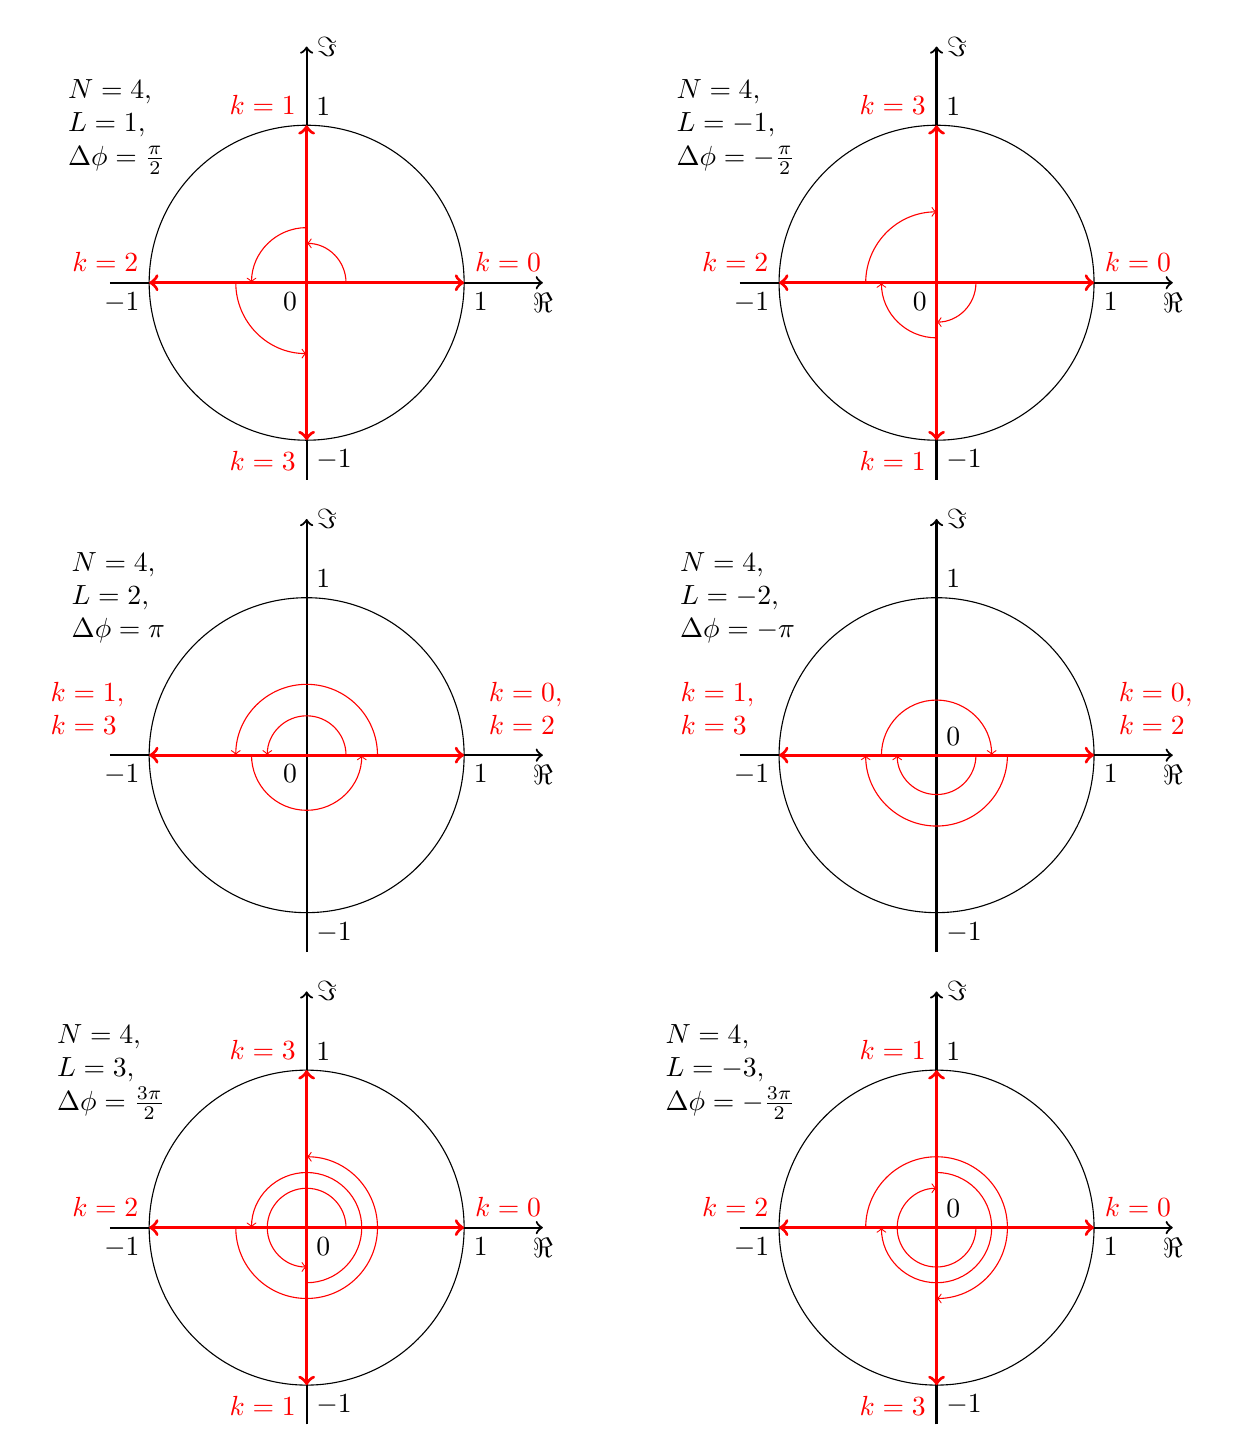
\begin{tikzpicture}
\draw (3cm,		-3cm)	circle [radius=2cm];
\draw (3cm,		-9cm)  	circle [radius=2cm];
\draw (3cm,		-15cm)	circle [radius=2cm];
\draw (11cm,	-3cm)	circle [radius=2cm];
\draw (11cm,	-9cm) 	circle [radius=2cm];
\draw (11cm,	-15cm) 	circle [radius=2cm];



%\draw (1cm,		-1cm)  node[above left]{$k=2 x =5 \int x dx$} 

\coordinate [label=left:\textcolor{black}{$\begin{array}{lc} N = 4, \\ L = 1, \\ \Delta \phi = \frac{\pi}{2} \end{array}$}] (A00) at (1.5cm, -1cm);
\coordinate [label=left:\textcolor{black}{$\begin{array}{lc} N = 4, \\ L = -1, \\ \Delta \phi = -\frac{\pi}{2} \end{array}$}] (A01) at (9.5cm, -1cm);
\coordinate [label=left:\textcolor{black}{$\begin{array}{lc} N = 4, \\ L = 2, \\ \Delta \phi = \pi \end{array}$}] (A10) at (1.5cm, -7cm);
\coordinate [label=left:\textcolor{black}{$\begin{array}{lc} N = 4, \\ L = -2, \\ \Delta \phi =-\pi \end{array}$}] (A11) at (9.5cm, -7cm);
\coordinate [label=left:\textcolor{black}{$\begin{array}{lc} N = 4, \\ L = 3, \\ \Delta \phi = \frac{3\pi}{2} \end{array}$}] (A20) at (1.5cm, -13cm);
\coordinate [label=left:\textcolor{black}{$\begin{array}{lc} N = 4, \\ L = -3, \\ \Delta \phi = -\frac{3\pi}{2} \end{array}$}] (A21) at (9.5cm, -13cm);


    	
\draw[->,thick] (3cm,	-5.5cm)		-- +(0cm,5.5cm)	node[right] {$\Im$};
\draw[->,thick] (3cm,	-11.5cm)	-- +(0cm,5.5cm)	node[right] {$\Im$};
\draw[->,thick] (3cm,	-17.5cm)	-- +(0cm,5.5cm)	node[right] {$\Im$};
\draw[->,thick] (11cm,	-5.5cm)		-- +(0cm,5.5cm)	node[right] {$\Im$};
\draw[->,thick] (11cm,	-11.5cm) 	-- +(0cm,5.5cm)	node[right] {$\Im$};
\draw[->,thick] (11cm,	-17.5cm) 	-- +(0cm,5.5cm)	node[right] {$\Im$};

\draw[->,thick] (0.5cm,	-3cm)	-- +(5.5cm,0cm)	node[below] {$\Re$};
\draw[->,thick] (0.5cm,	-9cm)	-- +(5.5cm,0cm)	node[below] {$\Re$};
\draw[->,thick] (0.5cm,	-15cm)	-- +(5.5cm,0cm)	node[below] {$\Re$};
\draw[->,thick] (8.5cm,	-3cm)	-- +(5.5cm,0cm)   node[below] {$\Re$};
\draw[->,thick] (8.5cm,	-9cm)	-- +(5.5cm,0cm)	node[below] {$\Re$};
\draw[->,thick] (8.5cm,	-15cm)	-- +(5.5cm,0cm)	node[below] {$\Re$};


\draw[-,thin] (1cm,	-3cm)  node[below left] {$-1$}	-- ++(2cm,0cm) 	node[below left] {$0$}	-- ++(2cm,0cm)	node[below right] {$1$};
\draw[-,thin] (1cm,	-9cm)  node[below left] {$-1$}	-- ++(2cm,0cm)	node[below left] {$0$}	-- ++(2cm,0cm)	node[below right] {$1$};
\draw[-,thin] (1cm,	-15cm) node[below left] {$-1$}	-- ++(2cm,0cm)	node[below right] {$0$}	-- ++(2cm,0cm)	node[below right] {$1$};
\draw[-,thin] (9cm,	-3cm)  node[below left] {$-1$}	-- ++(2cm,0cm) 	node[below left] {$0$}  -- ++(2cm,0cm)	node[below right] {$1$};
\draw[-,thin] (9cm,	-9cm)  node[below left] {$-1$}	-- ++(2cm,0cm)	node[above right] {$0$}	-- ++(2cm,0cm)	node[below right] {$1$};
\draw[-,thin] (9cm,	-15cm) node[below left] {$-1$}	-- ++(2cm,0cm)	node[above right] {$0$}	-- ++(2cm,0cm)	node[below right] {$1$};




\draw[-,thin] (3cm,		-5cm	)  node[below right] {$-1$}	-- +(0cm,4cm)	node[above right] {$1$};
\draw[-,thin] (3cm,		-11cm	)  node[below right] {$-1$}	-- +(0cm,4cm)	node[above right] {$1$};
\draw[-,thin] (3cm,		-17cm	)  node[below right] {$-1$}	-- +(0cm,4cm)	node[above right] {$1$};
\draw[-,thin] (11cm,	-5cm	)  node[below right] {$-1$}	-- +(0cm,4cm)   node[above right] {$1$};
\draw[-,thin] (11cm,	-11cm	)  node[below right] {$-1$}	-- +(0cm,4cm)	node[above right] {$1$};
\draw[-,thin] (11cm,	-17cm	)  node[below right] {$-1$}	-- +(0cm,4cm)	node[above right] {$1$};

                                                  
                                                  
                                                  
\begin{scope}[line width=1pt, red]

\draw[<->,very thick]  (1cm,	-3cm)  node[above left]{$k=2$}
				--	 ++(2cm,	 0cm)
				-- 	 ++(2cm,	 0cm)  node[above right]{$k=0$};

\draw[<->,very thick] (1cm,		-9cm) node[above left]{$\begin{array}{lc} k=1, \\ k=3 \end{array}$}	
				--	++(2cm,		 0cm)
				-- 	++(2cm,		 0cm)  node[above right]{$\begin{array}{lc} k=0, \\ k=2 \end{array}$};

\draw[<->,very thick] (1cm,		-15cm) node[above left]{$k=2$} 	
				-- 	++(2cm,		  0cm)                        
				-- 	++(2cm,		  0cm) node[above right]{$k=0$};

\draw[<->,very thick] (9cm,		-3cm) node[above left]{$k=2$}                                       	
				-- 	++(2cm,		 0cm)                                                                
				-- 	++(2cm,		 0cm)  node[above right]{$k=0$};                                     
				                                                                                     
\draw[<->,very thick] (9cm,		-9cm) node[above left]{$\begin{array}{lc} k=1, \\ k=3 \end{array}$}	 	
				-- 	++(2cm,		 0cm)                                                                
				-- 	++(2cm,		 0cm)  node[above right]{$\begin{array}{lc} k=0, \\ k=2 \end{array}$};
				                                                                                     
\draw[<->,very thick] (9cm,		-15cm) node[above left]{$k=2$} 	                                     	
				-- 	++(2cm,		  0cm)                                                               
				-- 	++(2cm,		  0cm) node[above right]{$k=0$};                                     


\draw[<->,very thick] (3cm,		-5cm)	node[below left] {$k=3$}
				  -- +(0cm, 	 4cm)	node[above left] {$k=1$};



\draw[<->,very thick] (3cm,		-17cm) node[below left] {$k=1$} 	
				  -- +(0cm, 	  4cm) node[above left] {$k=3$};


\draw[<->,very thick] (11cm,	-5cm)		node[below left] {$k=1$} 	
				  -- +(0cm, 	 4cm) 		node[above left] {$k=3$};


\draw[<->,very thick] (11cm,	-17cm)		node[below left] {$k=3$} 	
				  -- +(0cm, 	  4cm) 		node[above left] {$k=1$};

                                                



\draw[->,  thin] (3.5cm,-3cm) arc [start angle=0, end angle=90, radius=5mm];
\draw[->,  thin] (3.0cm,-2.3cm) arc [start angle=90, end angle=180, radius=7mm];
\draw[->,  thin] (2.1cm,-3cm) arc [start angle=180, end angle=270, radius=9mm];


\draw[->,  thin] (3.5cm,-9cm) arc [start angle=0, end angle=180, radius=5mm];
\draw[->,  thin] (2.3cm,-9cm) arc [start angle=180, end angle=360, radius=7mm];
\draw[->,  thin] (3.9cm,-9cm) arc [start angle=0, end angle=180, radius=9mm];


\draw[->,  thin] (3.5cm,-15cm) arc [start angle=0, end angle=270, radius=5mm];
\draw[->,  thin] (3.0cm,-15.7cm) arc [start angle=-90, end angle=180, radius=7mm];
\draw[->,  thin] (2.1cm,-15cm) arc [start angle=-180, end angle=90, radius=9mm];


\draw[->,  thin] (11.5cm,-3cm) arc [start angle=0, end angle=-90, radius=5mm];
\draw[->,  thin] (11.0cm,-3.7cm) arc [start angle=-90, end angle=-180, radius=7mm];
\draw[->,  thin] (10.1cm,-3cm) arc [start angle=-180, end angle=-270, radius=9mm];
                                                 

\draw[->,  thin] (11.5cm,-9cm) arc [start angle=0, end angle=-180, radius=5mm];
\draw[->,  thin] (10.3cm,-9cm) arc [start angle=-180, end angle=-360, radius=7mm];
\draw[->,  thin] (11.9cm,-9cm) arc [start angle=0, end angle=-180, radius=9mm];


\draw[->,  thin] (11.5cm,-15cm) arc [start angle=0, end angle=-270, radius=5mm];
\draw[->,  thin] (11.0cm,-14.3cm) arc [start angle=90, end angle=-180, radius=7mm];
\draw[->,  thin] (10.1cm,-15cm) arc [start angle=180, end angle=-90, radius=9mm];

\end{scope}
 

%\draw (-3.5cm,0cm) -- (3.5cm,0cm); 
%\draw (0cm,-3.5cm) -- (0cm,3.5cm);
%\draw (0cm,0cm) circle [radius=3cm];

\end{tikzpicture}
\end {document}                                    
%\caption{Сумма комплексных экспонент} \label{dft:fig4}
%\end{center}
%\end{figure}
%\end{singlespacing}
